\documentclass[a4paper]{scrartcl}

% Language
\usepackage[british, ngerman]{babel}

% Font stuff and typesetting stuff
\usepackage[utf8]{inputenc}
\usepackage[T1]{fontenc}
\usepackage{microtype}

% Font
\usepackage{lmodern}

% Other
\usepackage{amsmath, amssymb}
\usepackage{gensymb}
\usepackage{csquotes}
\usepackage{float}
\usepackage{graphicx}
\usepackage{lipsum}
\usepackage[obeyDraft]{todonotes}

\usepackage[colorlinks]{hyperref}

\usepackage[
	backend = biber, % Sets biber as backend.
	style = authoryear-icomp, % Use [author, year] citing with ibid. when duplicate.
	maxbibnames = 3, % Truncate lists above 3 entries (e.g. names).
	minbibnames = 3, % Truncate to 3 entries (e.g. names).
	maxcitenames = 2,
	mincitenames = 1,
	%backref = true,
	giveninits=true, % See warning
]{biblatex}
\DeclareNameAlias{sortname}{family-given}
\renewcommand{\multinamedelim}{\addsemicolon\space}

\addbibresource{references.bib}

\setkomafont{captionlabel}{%
	\bfseries
}

% Dank Koma-Klasse
\renewcaptionname{ngerman}{\subsectionautorefname}{Abschnitt}
\renewcaptionname{ngerman}{\figureautorefname}{Abb.}
\renewcaptionname{ngerman}{\tableautorefname}{Tab.}

\usepackage[
	automark,
	headsepline,
%	headtopline,
%	footsepline
]{scrlayer-scrpage}
%\pagestyle{scrheadings}
\ihead{Ralf Morawe}
\ohead[\pagemark]{\pagemark}
\chead{Ideen für Masterarbeit}
\cfoot[]{}

\begin{document}

\section*{Idee 1: Augmented Navigation}

Heutzutage verwenden Menschen digitale Navigationssysteme, um von einem Ort zum nächsten zu gelangen.
Bei diesen Systemen handelt es sich um GPS-Geräte oder auch mobile Apps.
Allerdings sind diese Systeme nicht ohne Fehler.
\textcite{Lin2017} analysieren das Phänomen \enquote{Death by GPS}.
Dieses beschreibt negative Ereignisse, die in Folge von der Nutzung solches Systeme auftreten.
Dazu zählen sowohl Fehlinformationen durch das System sowie schwierige Bedienung durch die Nutzer.
Ein Ansatz um diese Navigation einfacher und sicherer zu machen ist, die bisher meist iterative Navigation durch die Referenzierung von Landzeichen als Orientierungshilfe zu erweitern \parencites{Fingas2018}{Wenig2017}.

\begin{figure}[h]
	\centering
	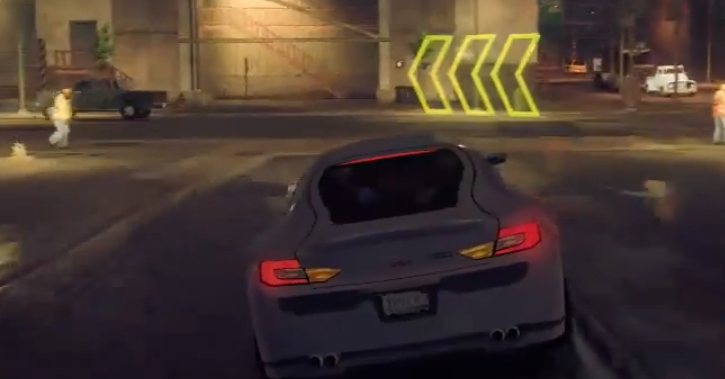
\includegraphics[width=0.6\textwidth]{figures/SR4GPS.png}
	\caption{In-Game GPS im Computerspiel \emph{Saints Row IV}. Der wegweisende Pfeil \enquote{schwebt} auf der Straße und zeigt die Richtung an.}
	\label{fig:sr4_gps}
\end{figure}

Auch in Spielen nimmt Navigation eine wichtige Rolle ein.
Ein interessanter Ansatz wird im Spiel \emph{Saints Row IV} präsentiert (siehe \autoref{fig:sr4_gps}).
Wenn Spieler einen Wegpunkt für ihre Ziele setzen, wird nicht nur auf einer Karte die kürzeste Route markiert.
Es werden zusätzliche Wegweiser an wichtigen Punkten der Straßenführung \emph{im direkten Sichtfeld} der Spieler angezeigt, wodurch die Navigation um einiges vereinfacht wird.

Dieses Prinzip kann dank neuer Augmented-Reality-Technologien (zum Beispiel die \emph{HoloLens} oder die \emph{Magic Leap} auf die Navigation in der realen Welt übertragen werden.
Das Ziel dieser Arbeit wäre es, eine landzeichen-basierte Navigation mithilfe dieser AR-Headsets zu implementieren.
Die Navigationshinweise würden dann (anstatt nur in 2D und/oder textueller Form) als Objekte im Sichtfeld der Nutzer angezeigt werden.
Von besonderem Interesse sind hier Einblendungen von Wegweisern sowie die Hervorhebung von Landzeichen.
Eine weitere Herausforderung könnte das Rendern dieser Objekte ohne Verdeckungen (\emph{Occlusion}) darstellen, was die Navigation negativ beeinflussen könnte.
Während \textcite{Walton2017} ein bildbasiertes Verfahren zur Verbesserung der Echtzeit-Verdeckungsberechnung vorschlagen, stellen \textcite{Kasperi2017} ein Verfahren vor, dass Umgebungsinformationen zur Rekonstruktion virtueller Gebäude und damit für die Berechnung verwendet.
Für diese Zwecke könnte auch die \emph{Google Maps API} genutzt werden \parencite{Google2018}.

%\begin{itemize}
%	\item \parencites[35--37]{vive2017}[88--120]{vive2017}[23]{vive2017}
%\end{itemize}

\section*{Idee 2: Cardboard Gesture Pack}
Es gibt inzwischen viele verschiedene AR/MR/VR-Headsets, die über Displays und Tracking-Technologien verfügen.
Aber auch im Niedrigpreissegment sind Lösungen erhältlich, die zum Beispiel ein Smartphone in ein solches Headset umwandeln können.
Die bekannteste ist Google Cardboard, bei dem ein Smartphone lediglich in ein Pappkonstrukt mit zwei einfachen Linsen gelegt wird.
Spezielle 360\degree Videos oder gerenderte Szenen können so einfach dargestellt werden.
Auch AR/MR ist durch Nutzen der Rückkamera des Smartphones möglich.
Vor allem für Anwendungen, bei denen eine große Zahl an Headsets notwendig ist (z.B. für Schulklassen oder allgemein Multi-User-AR/VR) ist diese günstige Lösung von Vorteil.

Diese Einfachheit beherbergt allerdings einen Nachteil:
da auf Controller sowie aufwendiges Tracking verzichtet wird, sind die Interaktionsmöglichkeiten mit den virtuellen Szenen begrenzt.
Lediglich die Kopfrotation sowie eine einfache \enquote{Tap}-Eingabe mittels Magnetschalter oder \enquote{\emph{Gaze-Input}} werden in der Regel unterstützt \parencite[vgl.][]{Yoo2015}.
Da Gaze-Input auf Dauer anstrengend ist und nicht immer geeignet ist, versuchen \textcite{Yan2016}, weitere Interaktionen über Antippen des Headsets zu implementieren.
Einige Geräte (z.B. das Moto G5) besitzen außerdem keinen Magnetometer, weshalb hier der einfache Schalter entfällt.
Die Idee des \emph{Cardboard Gesture Pack} wäre es, eine Reihe von verschiedenen Gesten mittels Bilderkennung zu ermitteln und diese für Interaktionen zu nutzen.
Diese Gesten könnten z.B. analog zu denen der HoloLens funktionieren.
\textcites{Xiao2018}{Harrison2011} zeigen, wie Gesten mithilfe von Tiefendaten der Headsets implementiert werden (siehe \autoref{fig:omnitouch}).
Da Smartphones in der Regel keine Tiefensensoren haben, wird hier die Erkennung weniger genau sein und ist daher limitiert.
Diese Limitierung könnte aber z.B. durch Anwenden des \emph{BinPut}-Verfahrens \parencite{Todi2017} umgangen werden, sodass auch mit simplen Gesten große Eingabemengen abgedeckt werden können.
Als Anwendung kann z.B. mit dem Gesture Pack das spiel \emph{Augmented Invaders} um zusätzliche Inhalte erweitert werden.
Aber auch andere Anwendungen sind denkbar.
Zum Beispiel könnte eine Screen-Sharing Lösung für Pair-Programming o.Ä. entwickelt werden.
Jeder AR-Nutzer hätte vor sich einen eigenen virtuellen Bildschirm.
Die Bildschirme aller Nutzer wären synchronisiert.
Kontrollieren ließen sich die Eingaben entweder über Tap-Gesten oder (falls zu ungenau) mit dem BinPut-Verfahren, welches auch für die Steuerung eines 2D-Cursors anwendbar ist.

\begin{figure}[h]
	\centering
	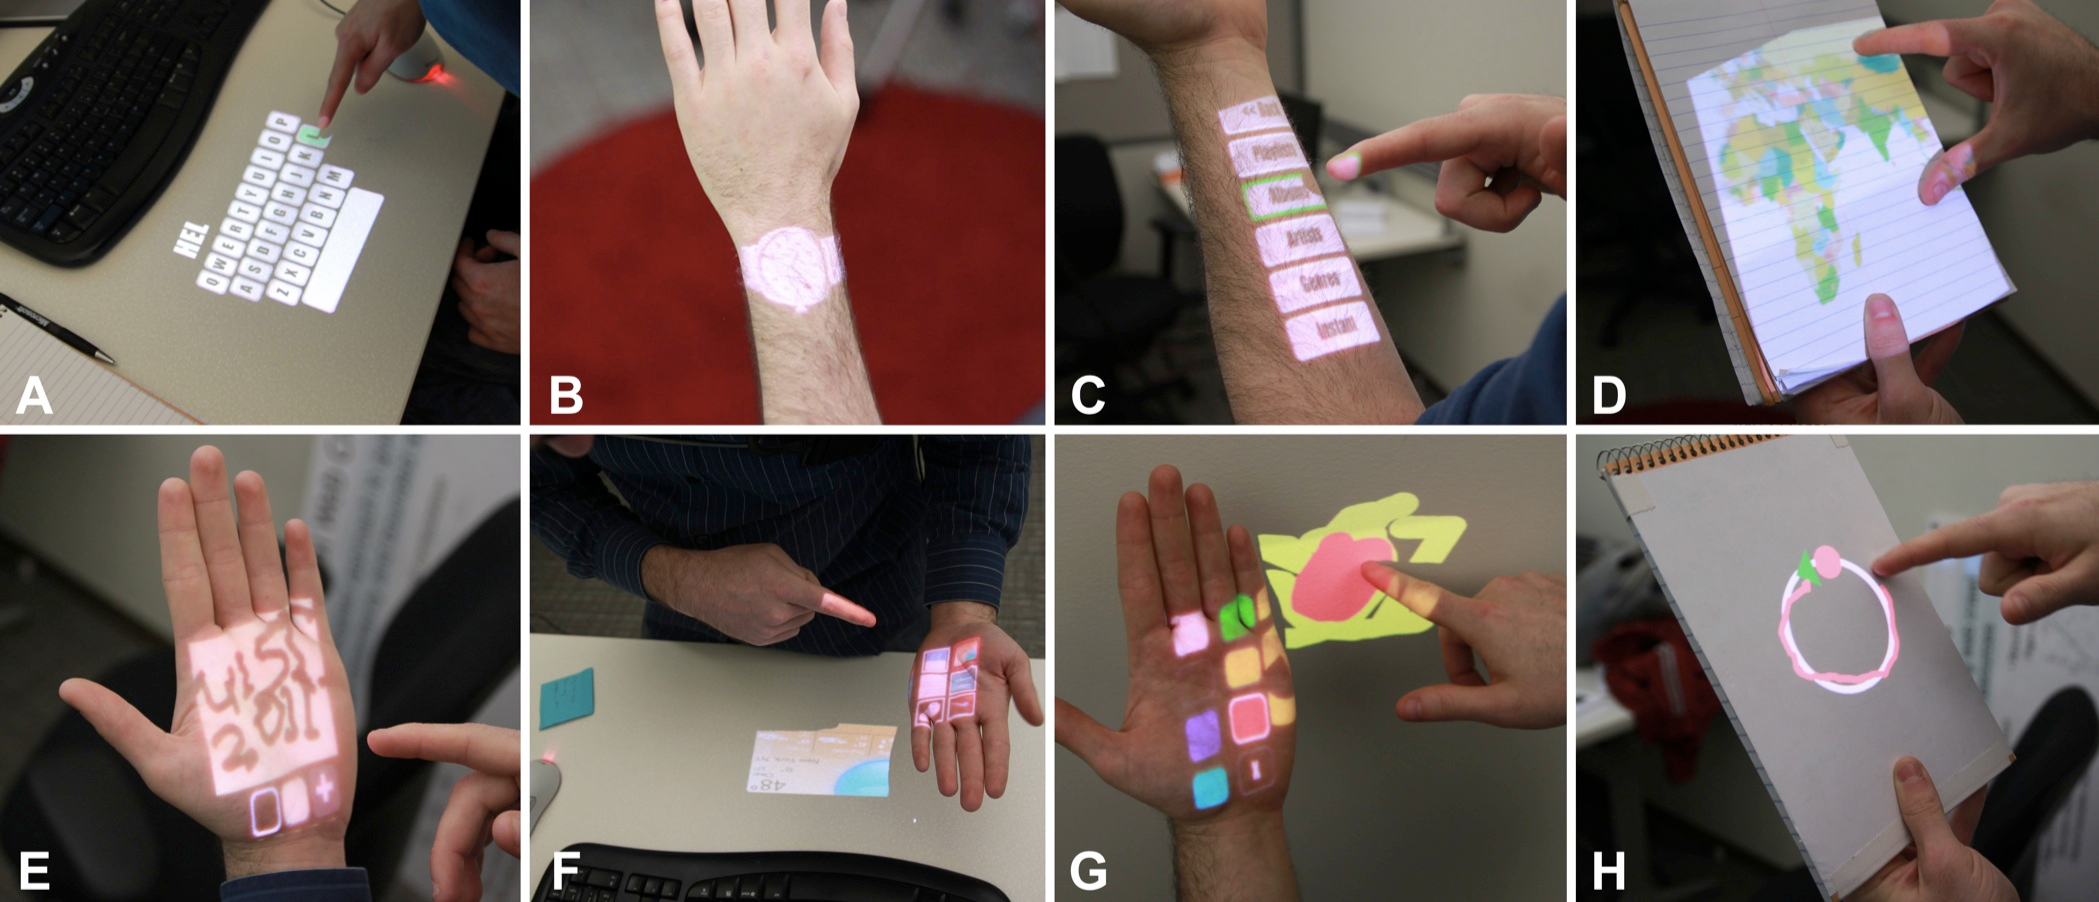
\includegraphics[width=\textwidth]{figures/omnitouch.png}
	\caption{Verschiedene Flächen werden für haptisches Feedback in MR eingesetzt. Die Berührungen werden mittels Gestenerkennung ermittelt. Quelle: \autocite{Harrison2011}}
	\label{fig:omnitouch}
\end{figure}

\section*{Idee 3: Dynamische Anzeige von Hindernissen in VR}
Das Anzeigen und Vermeiden von Hindernissen ist vor allem beim Multi-User-VR interessant, damit die verschiedenen Nutzer nicht kollidieren.
In der aktuellen Forschung werden dazu unterschiedliche Ansätze präsentiert.
Diese lassen sich meist in zwei Gruppen einteilen:
\begin{itemize}
	\item Die Kollisionen werden vermieden durch eine Aufteilung des Arbeitsvolumens.
	\item Andere Nutzer werden in der virtuellen Welt angezeigt.
\end{itemize}
Für den letzteren Ansatz zeigen \textcite{Lacoche2017} unterschiedliche Darstellungsmöglichkeiten.
Allerdings werden dort nur Nutzer gezeigt, die selbst ein HMD tragen.
Falls sich andere Menschen oder gar Gegenstände im Arbeitsvolumen befinden werden diese nicht angezeigt.

Die Idee wäre, andere Nutzer und Gegenstände z.B. mittels Tiefenbildern zu ermitteln und in der virtuellen Szene zu visualisieren.
So könnte ein HMDs-Nutzer in der virtuellen Welt vor Hindernissen gewarnt werden.
Dadurch könnten HMDs auch in kleineren und/oder dichteren Arbeitsvolumen sicher verwendet werden.
Zusätzlich öffnet dies die Möglichkeit für Anwendungen mit Interaktionen zwischen HMD-Nutzern und Nicht-HMD-Nutzern (Beispiel-Anwendung?).
Auch eine Verknüpfung mit den in der aktuellen Forschung relevanten Proxy-Objekten für passives haptisches Feedback ist möglich.
Objekte, mit denen Kollisionen für haptisches Feedback \emph{erwünscht} ist, könnten in der virtuellen Welt speziell dargestellt werden, um dem Nutzer die Interaktionsmöglichkeit zu vermitteln.

\printbibliography[nottype=online]
\printbibliography[title={Online Referenzen}, type=online]

\end{document}
